\documentclass[]{article}
\usepackage{amsmath}
\usepackage{amsfonts}
\usepackage{amssymb}
\usepackage{algorithmic}
\usepackage{algorithm}
\usepackage{tikz}
\usepackage{graphicx}
\usepackage{mdframed}
\usepackage{paralist}
\usepackage{listings}

\definecolor{dkgreen}{rgb}{0,0.6,0}
\definecolor{gray}{rgb}{0.5,0.5,0.5}

\lstset{
  language=Python,
  breaklines=true,
  showstringspaces=false,
  frame=single,
  aboveskip=3mm,
  belowskip=3mm,
  columns=flexible,
  basicstyle={\small\ttfamily},
  numbers=none,
  numberstyle=\tiny\color{gray},
  keywordstyle=\color{blue},
  commentstyle=\color{gray},
  stringstyle=\color{dkgreen},
  breakatwhitespace=true,
  tabsize=3
}

\title{CAGD - Homework 5}
\author{Josefine St{\aa}l \& Erik Ackzell}

\begin{document}

\maketitle

\section*{Task 1}
In this task we convert between barycentric and homogeneous coordinates.\\
Consider the points \begin{equation*}
p_0 = \left(\begin{array}{c}
1\\
1\\
1
\end{array}\right), \quad
p_1 = \left(\begin{array}{c}
3\\
3\\
3
\end{array}\right), \quad
p_2 = \left(\begin{array}{c}
1\\
2\\
2
\end{array}\right)
\end{equation*}
and let \begin{equation*}
q_1=\left(\begin{array}{c}
0.25\\
0.25\\
0.5
\end{array}\right)
\end{equation*}
in barycentric coordinates with respect to $p_0, p_1, p_2$. We want to express $q_1$ in homogeneous coordinates.\\
First, we express $q_1$ in Cartesian coordinates \begin{equation*}
q_1 = 0.25p_0 + 0.25p_1 + 0.5p_2 = \left(\begin{array}{c}
0.25 + 1.5 + 0.25\\
0.25 + 1.5 + 0.5\\
0.25 + 1.5 + 0.5
\end{array}\right) = \left(\begin{array}{c}
2\\
2.25\\
2.25
\end{array}\right).
\end{equation*}
For any $\omega\in\mathbb{R}$, the homogeneous coordinates of $q_1$ are\begin{equation*}
q_1 = \left(\begin{array}{c}
2\omega\\
2.25\omega\\
2.25\omega\\
\omega
\end{array}\right),
\end{equation*}
which is what we wanted to determine.\\
Now let \begin{equation*}
q_2 = \left(\begin{array}{c}
5\\
4\\
4\\
3
\end{array}\right)
\end{equation*}
in homogeneous coordinates. We wish to express $q_2$ in barycentric coordinates with respect to $p_0, p_1, p_2$.\\
First, we express $q_2$ in Cartesian coordinates \begin{equation*}
q_2 = \frac{1}{3}\left(\begin{array}{c}
5\\
4\\
4
\end{array}\right).
\end{equation*}
We now want to determine the coefficients $a_0, a_1, a_2$ such that \begin{equation*}
\sum_{i=0}^{2}a_ip_i
\end{equation*}
and \begin{equation*}
\sum_{i=0}^{2}a_i=1.
\end{equation*}
This can be done by solving the linear equation system \begin{equation*}
\left(\begin{array}{ccc}
1 & 3 & 1\\
1 & 3 & 2\\
1 & 3 & 2\\
1 & 1 & 1
\end{array}\right)\left(\begin{array}{c}
a_0\\
a_1\\
a_2
\end{array}\right) = \frac{1}{3}\left(\begin{array}{c}
5\\
4\\
4\\
3
\end{array}\right),
\end{equation*}
which reduces to \begin{equation*}
\left(\begin{array}{ccc}
1 & 3 & 1\\
1 & 3 & 2\\
1 & 1 & 1
\end{array}\right)\left(\begin{array}{c}
a_0\\
a_1\\
a_2
\end{array}\right) = \frac{1}{3}\left(\begin{array}{c}
5\\
4\\
3
\end{array}\right).
\end{equation*}
The solution is given by \begin{equation*}
a_0 = 1, \quad a_1 = \frac{1}{3}, \quad a_2 = -\frac{1}{3},
\end{equation*}
so in barycentric coordinates with respect to $p_0, p_1, p_2$, \begin{equation*}
q_2 = \frac{1}{3}\left(\begin{array}{r}
3\\
1\\
-1
\end{array}\right),
\end{equation*}
which is what we wanted to determine.
%\begin{figure}[h!]
%	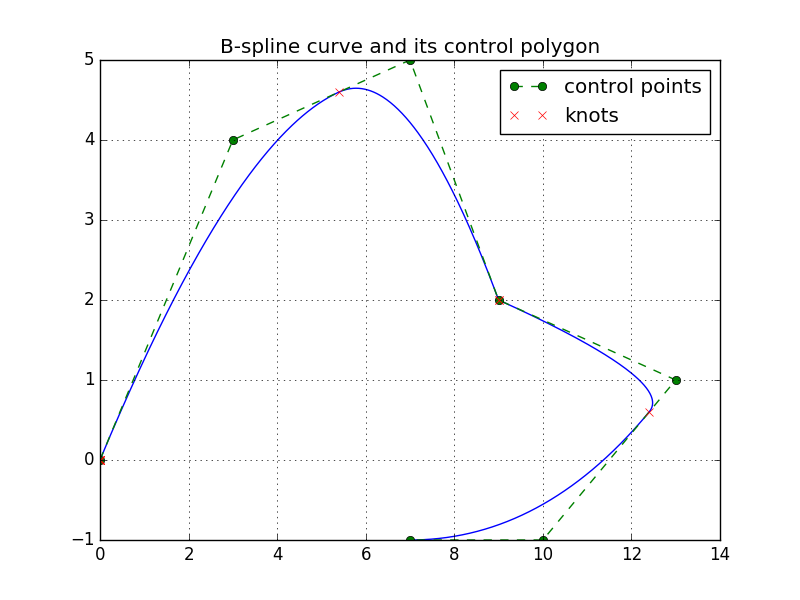
\includegraphics[scale=0.6]{bspline}
%\end{figure}

\section*{Do-over Homework 2 Task 5}
\underline{\textbf{Claim 1:}} The Lagrange form is invariant under all affine maps.\\
\\
\underline{\textbf{Proof:}} Let $\varphi:\mathbb{E}^n\rightarrow\mathbb{E}^n$ be any affine map. Then $\varphi$ can be expressed as \begin{equation*}
\varphi(u) = Au + v,
\end{equation*}
with $A\in\mathbb{R}^{n\times n}$ and $v\in\mathbb{R}^n$. Let $p$ be a polynomial of degree $n$. Then $p$ can be expressed as a linear combination of Lagrange basis polynomials $L_i^n$ of degree $n$, i.e. \begin{equation*}
p(x) = \sum_{i = 0}^{n}L_i^n(x)c_i,
\end{equation*}
with $c_i\in\mathbb{R}^n$ for $i = 0, 1, \dots, n$. Recall that the Lagrange basis fulfills the partition of unity, i.e. \begin{equation*}
\sum_{i = 0}^{n}L_i^n(x)=1.
\end{equation*}
We have that \begin{equation*}
\begin{aligned}
\varphi(p(x)) &= \varphi\left(\sum_{i = 0}^{n}L_i^n(x)c_i\right)\\
&= A\sum_{i = 0}^{n}L_i^n(x)c_i + v\\
&= \sum_{i = 0}^{n}L_i^n(x)Ac_i + v\\
&= \sum_{i = 0}^{n}L_i^n(x)Ac_i + 1\cdot v\\
&= \sum_{i = 0}^{n}L_i^n(x)Ac_i + \sum_{i = 0}^{n}L_i^n(x)v\\
&= \sum_{i = 0}^{n}L_i^n(x)(Ac_i + v)\\
&= \sum_{i = 0}^{n}L_i^n(x)\varphi(c_i)
\end{aligned}
\end{equation*}
which is what we wanted to show. $\square$\\
\\
\underline{\textbf{Corollary:}} The Lagrange form in invariant under all affine domain transformations.\\
\underline{\textbf{Proof:}} As all affine domain transformations are affine maps, the result follows directly from Claim 1. $\square$\\
\\
\underline{\textbf{Claim 2:}} The monomial form is \textbf{not} invariant under all affine domain transformation maps.\\
\\
\underline{\textbf{Proof:}} Let $\varphi:\mathbb{E}^n\rightarrow\mathbb{E}^n$ be any affine map. Then 
\newpage
\section*{Appendix I}
%\lstinputlisting[lastline=87]{bsplines.py}

\end{document}
